\documentclass[journal,12pt,twocolumn]{IEEEtran}

\usepackage{setspace}
\usepackage{gensymb}
\singlespacing
\usepackage[cmex10]{amsmath}

\usepackage{amsthm}

\usepackage{mathrsfs}
\usepackage{txfonts}
\usepackage{stfloats}
\usepackage{bm}
\usepackage{cite}
\usepackage{cases}
\usepackage{subfig}

\usepackage{longtable}
\usepackage{multirow}

\usepackage{enumitem}
\usepackage{mathtools}
\usepackage{steinmetz}
\usepackage{tikz}
\usepackage{circuitikz}
\usepackage{verbatim}
\usepackage{tfrupee}
\usepackage[breaklinks=true]{hyperref}
\usepackage{graphicx}
\usepackage{tkz-euclide}

\usetikzlibrary{calc,math}
\usepackage{listings}
    \usepackage{color}                                            %%
    \usepackage{array}                                            %%
    \usepackage{longtable}                                        %%
    \usepackage{calc}                                             %%
    \usepackage{multirow}                                         %%
    \usepackage{hhline}                                           %%
    \usepackage{ifthen}                                           %%
    \usepackage{lscape}     
\usepackage{multicol}
\usepackage{chngcntr}

\DeclareMathOperator*{\Res}{Res}

\renewcommand\thesection{\arabic{section}}
\renewcommand\thesubsection{\thesection.\arabic{subsection}}
\renewcommand\thesubsubsection{\thesubsection.\arabic{subsubsection}}

\renewcommand\thesectiondis{\arabic{section}}
\renewcommand\thesubsectiondis{\thesectiondis.\arabic{subsection}}
\renewcommand\thesubsubsectiondis{\thesubsectiondis.\arabic{subsubsection}}


\hyphenation{op-tical net-works semi-conduc-tor}
\def\inputGnumericTable{}                                 %%

\lstset{
%language=C,
frame=single, 
breaklines=true,
columns=fullflexible
}
\begin{document}

\newcommand{\BEQA}{\begin{eqnarray}}
\newcommand{\EEQA}{\end{eqnarray}}
\newcommand{\define}{\stackrel{\triangle}{=}}
\bibliographystyle{IEEEtran}
\raggedbottom
\setlength{\parindent}{0pt}
\providecommand{\mbf}{\mathbf}
\providecommand{\pr}[1]{\ensuremath{\Pr\left(#1\right)}}
\providecommand{\qfunc}[1]{\ensuremath{Q\left(#1\right)}}
\providecommand{\sbrak}[1]{\ensuremath{{}\left[#1\right]}}
\providecommand{\lsbrak}[1]{\ensuremath{{}\left[#1\right.}}
\providecommand{\rsbrak}[1]{\ensuremath{{}\left.#1\right]}}
\providecommand{\brak}[1]{\ensuremath{\left(#1\right)}}
\providecommand{\lbrak}[1]{\ensuremath{\left(#1\right.}}
\providecommand{\rbrak}[1]{\ensuremath{\left.#1\right)}}
\providecommand{\cbrak}[1]{\ensuremath{\left\{#1\right\}}}
\providecommand{\lcbrak}[1]{\ensuremath{\left\{#1\right.}}
\providecommand{\rcbrak}[1]{\ensuremath{\left.#1\right\}}}
\theoremstyle{remark}
\newtheorem{rem}{Remark}
\newcommand{\sgn}{\mathop{\mathrm{sgn}}}
\providecommand{\abs}[1]{\vert#1\vert}
\providecommand{\res}[1]{\Res\displaylimits_{#1}} 
\providecommand{\norm}[1]{\lVert#1\rVert}
%\providecommand{\norm}[1]{\lVert#1\rVert}
\providecommand{\mtx}[1]{\mathbf{#1}}
\providecommand{\mean}[1]{E[#1]}
\providecommand{\fourier}{\overset{\mathcal{F}}{ \rightleftharpoons}}
%\providecommand{\hilbert}{\overset{\mathcal{H}}{ \rightleftharpoons}}
\providecommand{\system}{\overset{\mathcal{H}}{ \longleftrightarrow}}
	%\newcommand{\solution}[2]{\textbf{Solution:}{#1}}
\newcommand{\solution}{\noindent \textbf{Solution: }}
\newcommand{\cosec}{\,\text{cosec}\,}
\providecommand{\dec}[2]{\ensuremath{\overset{#1}{\underset{#2}{\gtrless}}}}
\newcommand{\myvec}[1]{\ensuremath{\begin{pmatrix}#1\end{pmatrix}}}
\newcommand{\mydet}[1]{\ensuremath{\begin{vmatrix}#1\end{vmatrix}}}
\numberwithin{equation}{subsection}
\makeatletter
\@addtoreset{figure}{problem}
\makeatother
\let\StandardTheFigure\thefigure
\let\vec\mathbf
\renewcommand{\thefigure}{\theproblem}
\def\putbox#1#2#3{\makebox[0in][l]{\makebox[#1][l]{}\raisebox{\baselineskip}[0in][0in]{\raisebox{#2}[0in][0in]{#3}}}}
     \def\rightbox#1{\makebox[0in][r]{#1}}
     \def\centbox#1{\makebox[0in]{#1}}
     \def\topbox#1{\raisebox{-\baselineskip}[0in][0in]{#1}}
     \def\midbox#1{\raisebox{-0.5\baselineskip}[0in][0in]{#1}}
\vspace{3cm}
\title{AI1103 Assignment-1}
\author{V Rahul - AI20BTECH11030}
\maketitle
\newpage
\bigskip
\renewcommand{\thefigure}{\theenumi}
\renewcommand{\thetable}{\theenumi}
Download all python codes from 
\begin{lstlisting}
https://github.com/vrahul02/AI1103-Probability-and-Random-Variables/tree/main/Assignment-1/Codes
\end{lstlisting}
%
and latex-tikz codes from 
%
\begin{lstlisting}
https://github.com/vrahul02/AI1103-Probability-and-Random-Variables/tree/main/Assignment-1/Assignment-1.tex
\end{lstlisting}
\section*{Problem 1.5}
The probability that a student is not a swimmer is $\frac{1}{5}$.
Then the probability that out of five students, four are swimmers is\\\\
a) ${{5}\choose{4}}\times\left(\frac{4}{5}\right)^4\times\left(\frac{1}{5}\right)$\\
b) $\left(\frac{4}{5}\right)^4\times\left(\frac{1}{5}\right)$\\
c) ${{5}\choose{1}}\times\left(\frac{4}{5}\right)^4\times\left(\frac{1}{5}\right)$\\
d) None of these 
\section*{Solution}
Probability of 'non swimmer' = q = $\frac{1}{5}$\\
Since being 'swimmer' and being 'non swimmer' are mutually exclusive,\\
Probability of 'swimmer' = p = 1- q = $\frac{4}{5}$\\\\
Let K be a random variable representing number of students who are 'swimmer' in a given sample.\\
So K has a binomial distribution : 
\begin{align}
\Pr\brak{K=l} = {{n}\choose{l}} \times (q)^{n-l} \times (p)^{l}\label{0.0.1}
\end{align}
Where
\begin{itemize}
    \item n = Total number of students = 5
    \item p = Probability that a student is 'swimmer' = \( \frac{4}{5} \)
    \item q = Probability that a student is 'non swimmer' = \( \frac{1}{5} \)
    \item l= Total number of swimmers = 4
\end{itemize}
\bigskip
\begin{align}
\Pr\brak{K = 4}={{5}\choose{4}} \times\left(\frac{1}{5}\right)^{1} \times \left(\frac{4}{5}\right)^{4}\\\notag
\end{align}
As per the property of permutation and combination,
\begin{align}
{{n}\choose{l}}={{n}\choose{n-l}}\\
\implies\Pr\brak{K = 4}={{5}\choose{1}} \times\left(\frac{1}{5}\right)^{1} \times \left(\frac{4}{5}\right)^{4}\\\notag\\
\implies \Pr\brak{K = 4} = 0.4096\notag
\end{align}
Thus options a) and c) are correct\\
The probability that 4 students are 'swimmer' out of a random sample of 5 students is 0.4096.\\\\
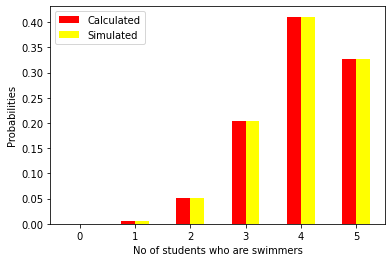
\includegraphics[width=100mm,scale=0.9]{Assignment-1.png}
\end{document}